\begin{figure}[H]
\centering
\includegraphics[page=6,width=0.48\textwidth]{\FCNCFigures/tthML/raw/faketau/prefit/NOMINAL/reg1l1tau1b1j_ss_vetobtagwp70_highmet/tau_pt_0.pdf}
\includegraphics[page=6,width=0.48\textwidth]{\FCNCFigures/tthML/raw/faketau/prefit/NOMINAL/reg1l1tau1b2j_ss_vetobtagwp70_highmet/tau_pt_0.pdf}
\includegraphics[page=6,width=0.48\textwidth]{\FCNCFigures/tthML/raw/faketau/prefit/NOMINAL/reg1l1tau1b2j_os_vetobtagwp70_highmet/tau_pt_0.pdf}
\includegraphics[page=6,width=0.48\textwidth]{\FCNCFigures/tthML/raw/faketau/prefit/NOMINAL/reg1l1tau1b3j_os_vetobtagwp70_highmet/tau_pt_0.pdf}
\includegraphics[page=6,width=0.48\textwidth]{\FCNCFigures/tthML/raw/faketau/prefit/NOMINAL/reg1l2tau1bnj_os/tau_pt_0.pdf}

\caption{轻子道信号区中$\tauhad$的$\pt$谱,图中的MC包含Fake tau的贡献,并且未经过任何Fake tau校准。可以看出其本底估计效果不理想。 }
\label{fig:pt_raw}
\end{figure}
